% Options for packages loaded elsewhere
\PassOptionsToPackage{unicode}{hyperref}
\PassOptionsToPackage{hyphens}{url}
\documentclass[
  11pt,
]{article}
\usepackage{xcolor}
\usepackage[a4paper, margin=2cm]{geometry}
\usepackage{amsmath,amssymb}
\setcounter{secnumdepth}{-\maxdimen} % remove section numbering
\usepackage{iftex}
\ifPDFTeX
  \usepackage[T1]{fontenc}
  \usepackage[utf8]{inputenc}
  \usepackage{textcomp} % provide euro and other symbols
\else % if luatex or xetex
  \usepackage{unicode-math} % this also loads fontspec
  \defaultfontfeatures{Scale=MatchLowercase}
  \defaultfontfeatures[\rmfamily]{Ligatures=TeX,Scale=1}
\fi
\usepackage{lmodern}
\ifPDFTeX\else
  % xetex/luatex font selection
\fi
% Use upquote if available, for straight quotes in verbatim environments
\IfFileExists{upquote.sty}{\usepackage{upquote}}{}
\IfFileExists{microtype.sty}{% use microtype if available
  \usepackage[]{microtype}
  \UseMicrotypeSet[protrusion]{basicmath} % disable protrusion for tt fonts
}{}
\makeatletter
\@ifundefined{KOMAClassName}{% if non-KOMA class
  \IfFileExists{parskip.sty}{%
    \usepackage{parskip}
  }{% else
    \setlength{\parindent}{0pt}
    \setlength{\parskip}{6pt plus 2pt minus 1pt}}
}{% if KOMA class
  \KOMAoptions{parskip=half}}
\makeatother
\usepackage{graphicx}
\makeatletter
\newsavebox\pandoc@box
\newcommand*\pandocbounded[1]{% scales image to fit in text height/width
  \sbox\pandoc@box{#1}%
  \Gscale@div\@tempa{\textheight}{\dimexpr\ht\pandoc@box+\dp\pandoc@box\relax}%
  \Gscale@div\@tempb{\linewidth}{\wd\pandoc@box}%
  \ifdim\@tempb\p@<\@tempa\p@\let\@tempa\@tempb\fi% select the smaller of both
  \ifdim\@tempa\p@<\p@\scalebox{\@tempa}{\usebox\pandoc@box}%
  \else\usebox{\pandoc@box}%
  \fi%
}
% Set default figure placement to htbp
\def\fps@figure{htbp}
\makeatother
\setlength{\emergencystretch}{3em} % prevent overfull lines
\providecommand{\tightlist}{%
  \setlength{\itemsep}{0pt}\setlength{\parskip}{0pt}}
\setmainfont{Times New Roman}
\usepackage[linesnumbered,ruled,vlined]{algorithm2e}
\usepackage{float}
\usepackage{amsmath}
\usepackage{amsfonts}
\usepackage{amssymb}
\usepackage{graphicx}
\usepackage{cite}
\usepackage{url}
\usepackage{hyperref}
\usepackage{bookmark}
\IfFileExists{xurl.sty}{\usepackage{xurl}}{} % add URL line breaks if available
\urlstyle{same}
\hypersetup{
  pdftitle={Image Informatics - 240150459},
  pdfauthor={Varsha Venkataraman},
  hidelinks,
  pdfcreator={LaTeX via pandoc}}

\title{Image Informatics - 240150459}
\author{Varsha Venkataraman}
\date{2025-01-08}

\begin{document}
\maketitle

\section*{\underline{Task 01 \textendash{} Image Reading and Displaying}}

\subsubsection*{\underline{Brief Introduction}}

As highlighted in {[}11{]}, understanding the fundamentals of image file
formats {[}1{]} and implementing efficient file readers significantly
enhances performance in image manipulation tasks. By applying similar
principles {[}12{]}, {[}13{]}, this algorithm outlines the process of
reading and displaying a PGM (Portable Gray Map) image using custom
functions, supporting future applications in digital image processing
and computer vision.

\subsubsection*{\underline{Algorithm for Image Reading and Displaying}}

\textbf{Step 1}: Call \texttt{process\_image()} and validate
\texttt{.pgm} extension with \texttt{validate\_pgm\_file()}.\\
\textbf{Step 2}: If valid, call \texttt{image\_read()} to read header
info (magic number, width, height, max value). If any line exceeds 70
characters, throw an error.\\
\textbf{Step 2.1}: If magic number is \texttt{'P5'}, call
\texttt{process\_pgm\_noisyImage()} for binary PGM, else process ASCII
PGM.\\
\textbf{Step 3a}: For ASCII PGM, initialize \texttt{warning\_count = 0}.
Decode lines, strip whitespace, skip comments.\\
\textbf{Step 3.1}: If lines exceed 70 characters, increment
\texttt{warning\_count} and throw a warning.\\
\textbf{Step 3.2}: Call \texttt{read\_pgm\_header()} for width, height,
\texttt{max\_value}, and \texttt{pixel\_lines}.\\
\textbf{Step 3.3}: Validate pixel data, apply gamma correction, reshape
pixels, and return the image.\\
\textbf{Step 3b}: For \texttt{'P5'}, call
\texttt{process\_pgm\_noisyImage()} and read binary data.\\
\textbf{Step 3.1}: Call \texttt{read\_binary\_lines()} to extract header
and pixel data, validate, apply gamma correction, reshape, and return
the image.\\
\textbf{Step 4}: If header exceeds 70 characters, throw an error:
``Header exceeds 70 characters.''\\
\textbf{Step 5}: Return and display the processed image.

\subsubsection*{\underline{Key Findings}}

\begin{itemize}
    \item \textbf{Format Validation:} Successfully differentiated between P2 (ASCII) and P5 (Binary) PGM formats, handled the header information ensuring robust input handling for both types.
    \item \textbf{Custom Implementation:} Implemented a detailed algorithm for reading and processing PGM files, demonstrating an understanding of file handling and image processing concepts.
    \item \textbf{Gamma Correction:} Applied gamma correction to adjust pixel intensity levels, improving image representation for visualization.[1]
\end{itemize}

\subsubsection*{\underline{Results and Conclusion}}

\begin{itemize}
        \item Successfully processed and displayed a the provided PGM image file. The pixel intensities were accurately read, reshaped, and visualized.
        \item  Validated file formats and handled invalid formats with appropriate errors. Algorithm handled images of varying sizes and formats efficiently. Displayed with clear intensity differentiation and enhanced visibility through gamma correction.
    \item \textbf{Robust Workflow and learning outcome:} The algorithm ensures correctness and efficiency in processing PGM images.Gained a deeper understanding of image file formats, header parsing, data validation, and visualization techniques.
\end{itemize}

\subsubsection*{\underline{Flow Chart}}
\begin{figure}[H]
\centering
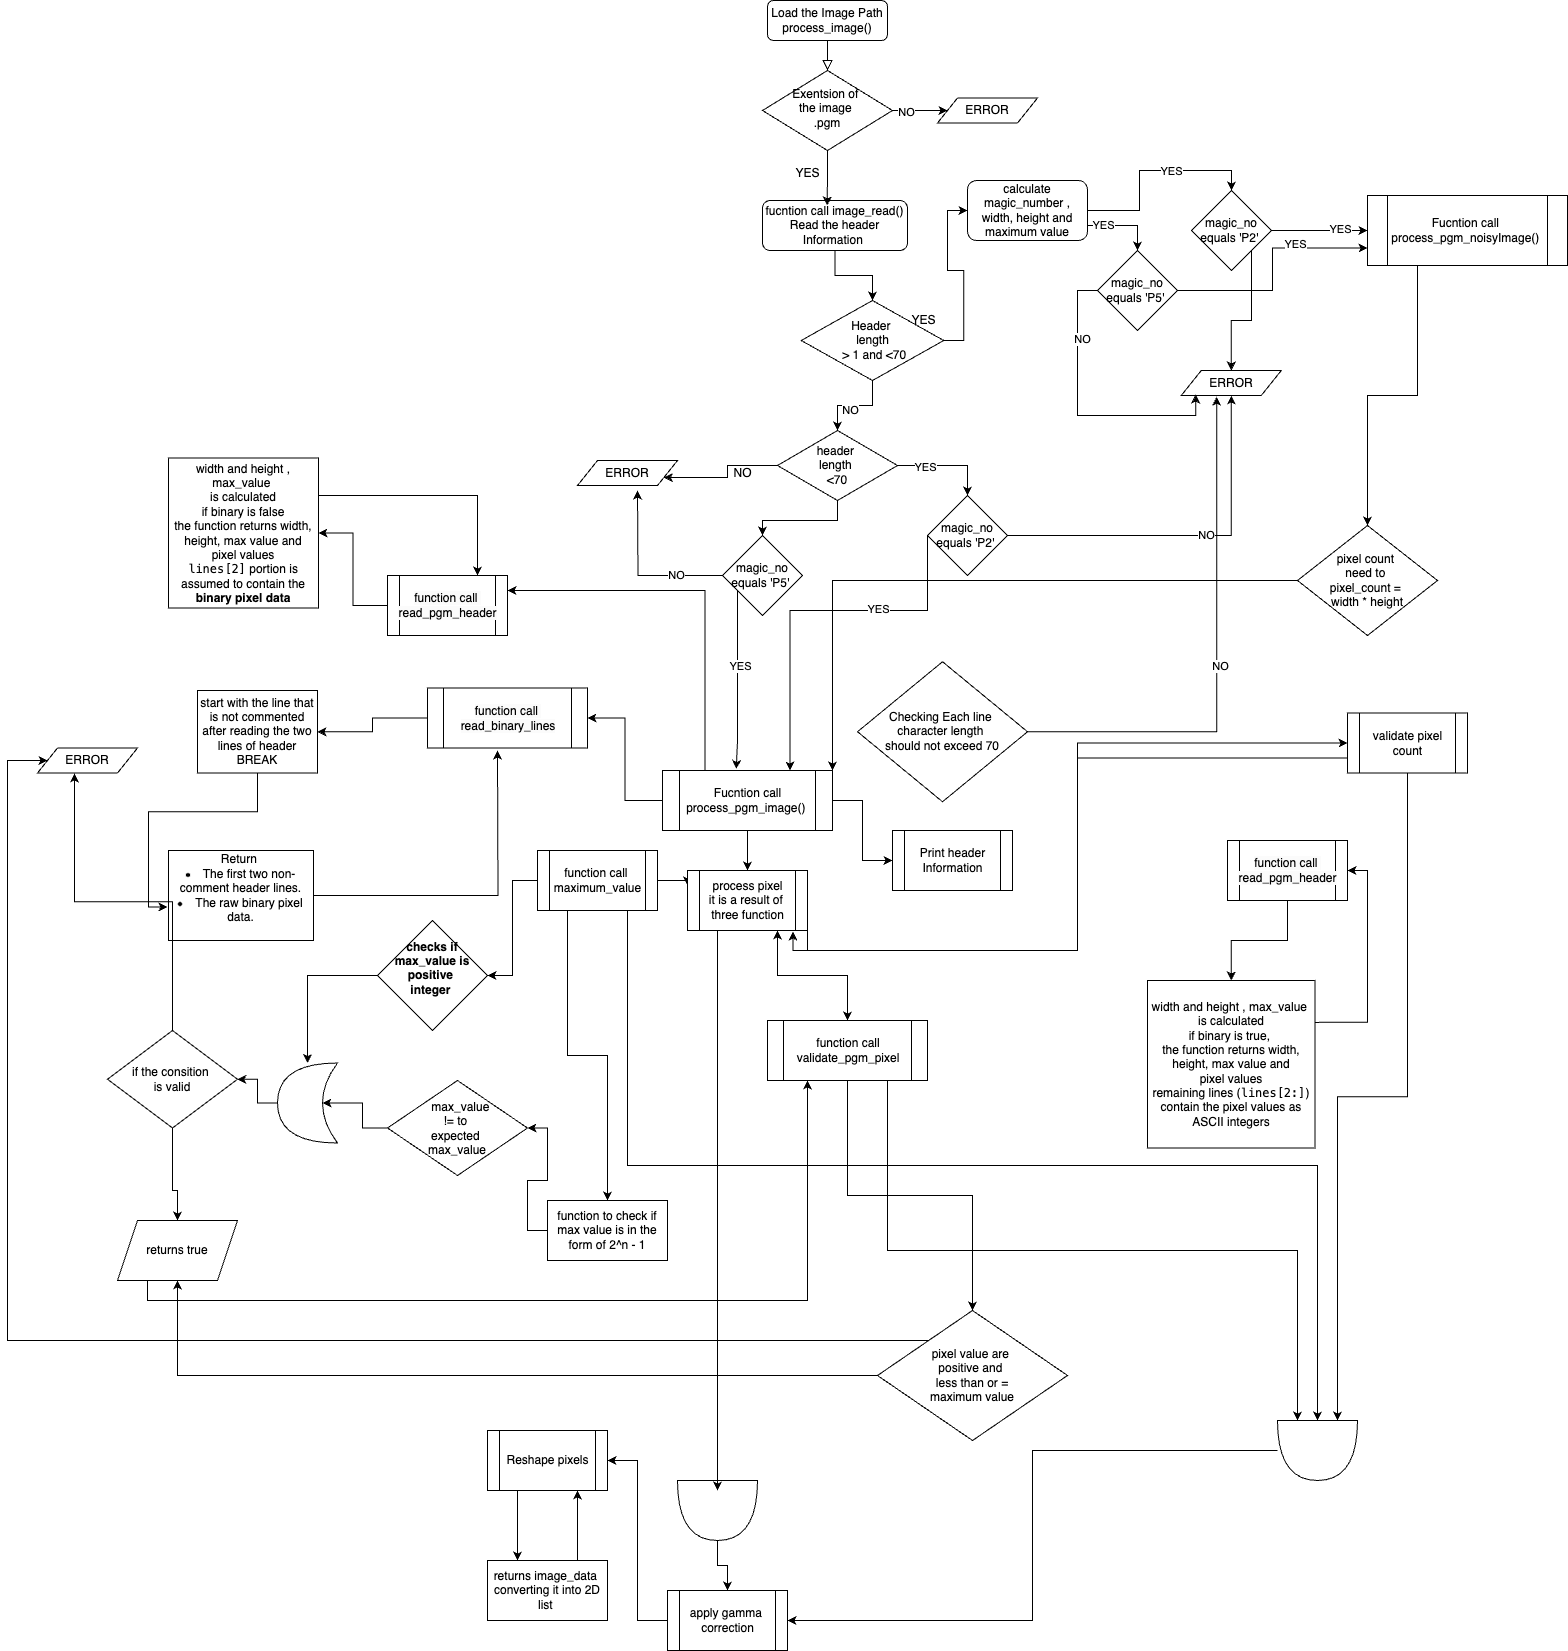
\includegraphics[width=\textwidth,height=\textheight,keepaspectratio]{~/Downloads/pgm.png}
\caption{Flowchart illustrating the PGM processing algorithm.}
\label{fig:flowchart}
\end{figure}

\subsubsection*{\underline{Output}}
\begin{figure}[H]
\centering
\includegraphics[width=0.4\textwidth,height=0.4\textheight,keepaspectratio]{~/Downloads/original.jpeg}
\caption{Output of Image by read function.}
\label{fig:flowchart}
\end{figure}

\section*{\underline{Task 02 \textendash{} Wavelet decomposition}}

\subsubsection*{\underline{Brief Introduction}}

Wavelet transformation is a powerful technique for analyzing and
processing images, providing multi-resolution decomposition of data. It
allows the separation of an image into approximation and detail
coefficients, enabling efficient compression, denoising, and feature
extraction{[}14{]}. This algorithm explores the implementation of
wavelet decomposition and reconstruction for image processing.

\textbf{Input:} A 2D numpy array representing the grayscale image. with
number of levels for the Forward Discrete Wavelet Transform (FDWT).
{[}15{]}

\textbf{Output:} Approximation and detail coefficients (horizontal,
vertical, diagonal).{[}15{]} and The original image reconstructed from
the decomposed coefficients using the Inverse Discrete Wavelet Transform
(IDWT).

\subsubsection*{\underline{Algorithm for Haar Wavelet Transformation and Image Reconstruction}}

\textbf{Step 1:} Pad the Image Data as Haar deals with even dimension
{[}15{]}, Check if the dimensions (rows and columns) of the image are
even. If the dimensions are odd, pad the array with zeros to make both
dimensions even.

\textbf{Step 2:} Perform Forward Discrete Wavelet Transform (FDWT)\\
-\textbf{Step 2.1:} For each level of decomposition: Apply the 1D Haar
wavelet filter: {[}14{]} \[
          \text{Low-pass filter output} = \frac{x_{2n} + x_{2n+1}}{sqrt(2)}, \quad            \text{High-pass filter output} = \frac{x_{2n} - x_{2n+1}}{sqrt(2)}
        \] For each row: Compute low-pass and high-pass filtered values,
For each column: Compute low-pass and high-pass filtered values.

-\textbf{Step 2.2:} Combine results into four components, Approximation
,Horizontal Details, Vertical Details, Diagonal Details

-\textbf{Step 2.3:} Store the detail coefficients (horizontal, vertical,
diagonal) and update the approximation for the next level.

-\textbf{Step 3:} Perform Inverse Discrete Wavelet Transform (IDWT)\\
-\textbf{Step 3.1:} For each level in reverse: Combine the approximation
and detail coefficients into a single matrix.\\
-\textbf{Step 3.1.1:} Apply the inverse Haar wavelet filter: For each
column: Reconstruct the original column from low-pass and high-pass
components. For each row: Reconstruct the original row from low-pass and
high-pass components.

-\textbf{Step 3.2:} Update the approximation until the original image
dimensions are restored.\\
-\textbf{Step 4:} Perform IDWT on the decomposed coefficients to
reconstruct the image.\\
\hspace{2cm} The Inverse Discrete Wavelet Transform (IDWT) reconstructs
the original image by combining the approximation (low-pass) and detail
(high-pass) coefficients.

-\textbf{Step 5:} Display the reconstructed image using a grayscale
colormap (\texttt{cmap=\textquotesingle{}gray\textquotesingle{}}).

-\textbf{Step 6:} Calculate the Mean Squared Error (MSE) between the
original and reconstructed images.\\
\[
\text{MSE} = \frac{1}{N} \sum_{i=1}^{N} (x_{\text{original},i} - x_{\text{reconstructed},i})^2
\] Evaluate the wavelet decomposition's quality based on the MSE value.

\subsubsection*{\underline{Key Findings and results}}

The results of the forward and inverse discrete wavelet transform (FDWT
and IDWT) show that the Haar wavelet filter effectively decomposes the
image into approximation and detail coefficients across multiple levels.

\begin{figure}[H]
\centering
\includegraphics[width=0.4\textwidth,height=0.4\textheight,keepaspectratio]{~/Downloads/wavelettransform.jpeg}
\caption{Output of Image by read function.}
\label{fig:flowchart}
\end{figure}

After applying the inverse transform (IDWT), the image is successfully
reconstructed, with minimal loss of information. The computed Mean
Squared Error (MSE) between the original and reconstructed image
confirms the efficiency of the wavelet transform, with very low values
indicating accurate reconstruction.The computed Mean Squared Error (MSE)
between the original and reconstructed image confirms the efficiency of
the wavelet transform, with very low values indicating accurate
reconstruction.

\begin{figure}[H]
\centering
\includegraphics[width=0.4\textwidth,height=0.4\textheight,keepaspectratio]{~/Downloads/comparison.jpeg}
\caption{Output of Image by read function.}
\label{fig:flowchart}
\end{figure}

\subsubsection*{\underline{Flow Chart}}
\begin{figure}[H]
\centering
\includegraphics[width=\textwidth,height=\textheight,keepaspectratio]{~/Downloads/task2.png}
\caption{Flowchart illustrating forward wavelet decomposition algorithm.}
\label{fig:flowchart}
\end{figure}

\begin{figure}[H]
\centering
\includegraphics[width=\textwidth,height=\textheight,keepaspectratio]{~/Downloads/inverse.jpg}
\caption{Flowchart illustrating inverse wavelet decomposition algorithm.}
\end{figure}

\begin{figure}[H]
\centering
\includegraphics[width=0.8\textwidth]{~/Desktop/IINFO/mse.png}
\caption{Flowchart illustrating MSE calculation algorithm.}
\end{figure}

\subsubsection*{\underline{Discussions and Conclusions}}

The Haar wavelet decomposition provides a simple yet powerful technique
for multi-level image compression and analysis. The low MSE values
demonstrate that the FDWT and IDWT are working as expected, preserving
the key features of the original image. This method can be further
optimized and applied in various image processing tasks, such as
denoising, compression, and feature extraction, while maintaining
computational efficiency.

\section*{\underline{Task 03 \textendash{} Image Denoising }}

\subsubsection*{\underline{Brief Introduction}}

The primary goal of denoising is to recover a clean image from a noisy
one while preserving essential details. Various types of noise, such as
Gaussian, salt-and-pepper, and impulse noise, necessitate diverse
denoising strategies {[}4{]}. The Wavelet Transform (WT) is a powerful
tool for image denoising due to its multi-scale analysis capabilities.
Unlike spatial domain methods, WT operates in the frequency domain,
allowing effective noise separation and feature preservation. Classic
methods like VisuShrink use WT to compute adaptive noise suppression
thresholds, significantly improving denoising performance {[}3{]}.
Recent hybrid strategies combine wavelet-based denoising with median
filtering, Gaussian filtering, and total variation minimization to
address limitations of individual methods, enhancing overall denoising
effectiveness.

\subsubsection*{\underline{Algorithm: Image Denoising using Wavelet Transform}}

-\textbf{Step 1:} Initialize Parameters, Set wavelet level to 3, filter
strength \texttt{nlm\_h} to 0.4, and TV denoising weight
\texttt{tv\_weight} to 0.1.

-\textbf{Step 2:} Classify image noise as impulse or Gaussian.

-\textbf{Step 3:} Apply median filter to remove impulse noise by
replacing each pixel with the median value from its neighborhood.

-\textbf{Step 4:} Apply Gaussian filter to smooth image and remove
Gaussian noise by averaging pixel values with a Gaussian kernel.

-\textbf{Step 5:} Perform wavelet decomposition and separate noise at
multiple scales.\\
- Classify noise (`salt and pepper' or `Gaussian').\\
- Apply median filtering for `salt and pepper' and Gaussian filtering
for `Gaussian' noise.\\
- Perform thresholding using VisuShrink on wavelet coefficients and
reconstruct the image.\\
- Apply Non-Local Means Denoising by averaging similar patches with
filter strength \texttt{nlm\_h}.\\
- Apply Total Variation Denoising for edge-preserving smoothing using
\texttt{tv\_weight}.

-\textbf{Step 6:} Predefined Wavelet Denoising Methods ,Use VisuShrink
with a universal threshold based on noise levels.

-\textbf{Step 7:} Return the denoised image close to the original clean
image.

-\textbf{Step 8:} Apply adaptive weight fusion {[}18{]}, {[}19{]} using
wavelet denoising, mean filtering, and median filtering outputs to get a
fused denoised image.

-\textbf{Step 9:} Calculate MSE between original and denoised images.

-\textbf{Step 10:} Compute Structural Similarity Index:\\
\[
\text{SSIM}(I, K) = \frac{(2\mu_I \mu_K + c_1)(2\sigma_{IK} + c_2)}{(\mu_I^2 + \mu_K^2 + c_1)(\sigma_I^2 + \sigma_K^2 + c_2)}
\]

\subsubsection*{\underline{Key findings:}}

The proposed algorithm effectively denoises images, preserving critical
structures while removing noise. Unlike the mean and median filters,
which introduce blurring and detail loss, the fusion method retains
edges and fine textures more effectively. The custom wavelet denoising,
which incorporates dynamic thresholding and adaptive fusion, outperforms
the predefined wavelet methods.

This combined approach shows excellent noise reduction for both Gaussian
and impulse noise, common in medical imaging. It excels at preserving
edges, textures, and key anatomical structures, especially in boundary
regions, confirming its effectiveness for medical image denoising
{[}4{]}, {[}5{]}, {[}6{]}.

\subsubsection*{\underline{Result:}}

With respect to the attached below figure (8), the fusion image acheived
the lowest MSE value and the highest SSIM value when compared with the
traditional filters and standalone wavelet denoising algorithm. The
method preserves the fine details in the medical images, particularly
the bone stuctures, while significantly suppresing noise without
over-smoothing when compared with the mean and median filters.The
results confirm that the adaptive wavelet-based fusion outperforms the
individual methods in both qualitative and visual metrics and quality.

\begin{figure}[H]
\centering
\includegraphics[width=0.5\textwidth,height=0.5\textheight,keepaspectratio]{~/Downloads/valueresult.jpeg}
\caption{Comparison metrics}
\end{figure}

\subsubsection*{\underline{Image Denoising Flowchart }}
\begin{figure}[H]
\centering
\includegraphics[width=\textwidth,height=\textheight,keepaspectratio]{~/Downloads/task3.png}
\caption{Flowchart illustrating Image Denoising algorithm.}
\end{figure}

\subsubsection*{\underline{Conclusion:}}
\begin{figure}[H]
\centering
\includegraphics[width=0.5\textwidth,height=0.5\textheight,keepaspectratio]{~/Downloads/result.jpeg}
\end{figure}

The combined denoising approach maintains a balance between the noise
supression and detail preservation. The weighted averaging fusion (or
Weighted image fusion) effectively leverages the strengths of each
denoising method, resulting in a denosied image that retains the
important features such as edges, textures and other fine details.
Future work could focus on further optimizing the fusion process by
experimenting with more advanced optimization techniques, such as
machine learning-based weight selection and deep learnig approach
{[}7{]}.

\renewcommand{\refname}{\textbf{References}}
\begin{thebibliography}{}

\bibitem{pgm_specification} 
Netpbm Documentation, "PGM (Portable Gray Map) image format specification," 2024. [Online]. Available: \url{https://netpbm.sourceforge.net/doc/pgm.html}. [Accessed: Dec. 28, 2024].

\bibitem{5231532} 
L. Hongqiao and W. Shengqian, "A new image denoising method using wavelet transform," in  \textit{Proc. 2009 Int. Forum Inf. Technol. Appl.}, 2009, pp. 111–114, doi: 10.1109/IFITA.2009.47.

\bibitem{article} 
B. K. S. Kumar, "Image denoising based on non-local means filter and its method noise thresholding,"  \textit{Signal, Image Video Process.}, vol. 7, pp. 1211–1227, Nov. 2013, doi: 10.1007/s11760-012-0389-y.

\bibitem{5364696}
G. Xi, W. Sun, and L. Ma, "Mixed wavelet and median filter for image denoising," in  \textit{Proc. 2009 Int. Conf. Comput. Intell. Softw. Eng.}, 2009, pp. 1–4, doi: 10.1109/CISE.2009.5364696.

\bibitem{6780128}
A. Boyat and B. K. Joshi, "Image denoising using wavelet transform and median filtering," in  \textit{Proc. 2013 Nirma Univ. Int. Conf. Eng. (NUiCONE)}, 2013, pp. 1–6, doi: 10.1109/NUiCONE.2013.6780128.

\bibitem{7396441}
Q. Song, L. Ma, J. Cao, and X. Han, "Image denoising based on mean filter and wavelet transform," in  \textit{Proc. 2015 4th Int. Conf. Adv. Inf. Technol. Sens. Appl. (AITS)}, 2015, pp. 39–42, doi: 10.1109/AITS.2015.17.

\bibitem{liu2023}
C. Liu and L. Zhang, "A novel denoising algorithm based on wavelet and non-local moment mean filtering,"  \textit{Electronics}, vol. 12, no. 6, p. 1461, 2023, doi: 10.3390/electronics12061461.

\bibitem{parmar2013}
P. L. Parmar, "Image denoising using VisuShrink algorithm," \textit{Vishwakarma Gov. Eng. Coll. J.}, vol. 2, no. 2, pp. 762–764, 2013.

\bibitem{1467423}
A. Buades, B. Coll, and J.-M. Morel, "A non-local algorithm for image denoising," in \textit{Proc. IEEE Comput. Soc. Conf. Comput. Vis. Pattern Recognit. (CVPR)}, vol. 2, 2005, pp. 60–65, doi: 10.1109/CVPR.2005.38.

\bibitem{dd1519c0884743e0848e32a61c483198} 
M. Mittermary, S. G. Nikolov, H. Hutter, and M. Grasserbauer, "Wavelet de-noising of Gaussian peaks: A comparative study," \textit{Chemometrics and Intelligent Laboratory Systems}, vol. 34, pp. 187--202, 1996.

\bibitem{article} 
S. Pawar, P. Halgaonkar, J. W. Bakal, and V. M. Wadhai, 
"Implementation of PPM image processing and median filtering," 
\textit{International Journal of Computer Applications}, 
vol. 14, 2011. 
doi: 10.5120/1843-2489.

\bibitem 
Available: \url{https://ilkerbayram.github.io/ehb372e/HaarDWT/}

\bibitem
Available: \url{https://github.com/Tanu-N-Prabhu/Python/blob/master/Reading\_An\_Image\_In\_Python\_(Without\_Using\_
Special\_Libraries).ipynb}

\bibitem{}
C. S. Leung and S. Kulkarni, \url{"Implementation of wavelet decomposition and reconstruction for an image using TMS320C6701}," \textit{Electrical Engineering Department, Texas A\&M University-Kingsville}, Kingsville, Texas 78363.

\bibitem{}
Available: \url{https://uk.mathworks.com/help/wavelet/ref/haart.html}

\bibitem{}
Available: \url{https://stackoverflow.com/questions/57439509/implementing-haar-wavelet-in-python-without-packages}

\bibitem {}
S. Kavitha and H. Inbarani, “COVID-19 and MRI Image Denoising Using Wavelet Transform and Basic Filtering,” 2021 5th International Conference on Intelligent Computing and Control Systems (ICICCS)

\bibitem{}
L. Song, Y. Lin, W. Feng, and M. Zhao, “A Novel Automatic Weighted Image Fusion Algorithm,” State Key Laboratory of Precision Measuring Technology and Instruments, Tianjin University.

\bibitem{}
G. Qi, G. Hu, N. Mazur, H. Liang, and M. Haner, “A Novel Multi-Modality Image Simultaneous Denoising and Fusion Method Based on Sparse Representation,”

\end{thebibliography}

\end{document}
